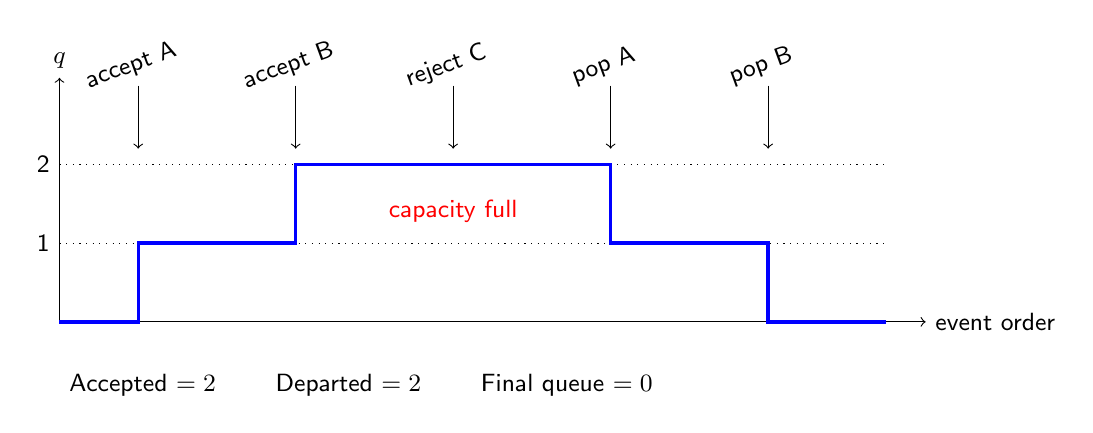
\begin{tikzpicture}[x=1cm,y=1cm,font=\small\sffamily]
\draw[->] (0,0)--(11,0) node[right] {event order};
\draw[->] (0,0)--(0,3.1) node[above] {$q$};
\foreach \y in {1,2} {\draw[dotted] (0,\y)--(10.5,\y);\node[left] at (0,\y) {\y};}
\draw[Blue,very thick] (0,0)--(1,0)--(1,1)--(3,1)--(3,2)--(7,2)--(7,1)--(9,1)--(9,0)--(10.5,0);
\foreach \x/\t in {1/accept A,3/accept B,5/reject C,7/pop A,9/pop B} {\draw[->] (\x,3)--(\x,2.2);\node[above,rotate=20] at (\x,3) {\t};}
\node[Red] at (5,1.4) {capacity full};
\node[anchor=west] at (0,-.8) {Accepted $=2$ \qquad Departed $=2$ \qquad Final queue $=0$};
\end{tikzpicture}
